\chapter{Simulation and Results}
\label{chap:5_Simulation_And_Results}
    
        In this chapter, we present scenarios for validation and evaluation and experimental results. The scenarios cover different encounters between vessels for collision avoidance evaluation and exposition to different wind speeds to identification of the system response and limitations. Beyond that, we present the execution with and without \ac{ATC} for scientific control evaluation of the path planning algorithm. As done by several authors, \eg{} Larson \etal{} ~\cite{Larson2006Autonomous}, Naeem \etal{} ~\cite{Naeem2012COLREGS}, Campbell \etal{} ~\cite{Campbell2013Automatic}, Naus ~\cite{Naus2013Idea}, \etc{}, we evaluated 4 main encounter scenarios between two vessels: head-on, crossing from right, crossing from left and overtaking;

    \section{Simulations Characterization}
    
    %DJ: Maybe show comparison between study simulation format and our
    Scenarios have been developed (Figure \ref{fig:simulation_uwsim_encounters}) to evaluate the system focusing on being comparable with scenarios presented in reference studies, \ie{} Agrawal \etal{} ~\cite{Agrawal2015COLREGS} and Huang \etal{} ~\cite{Huang2019Generalized}. Both studies were chosen for their quality and similarity with our work. Agrawal \etal{} was chosen for being our problem-solving inspiration, unfortunately, they do not present too much information about their system evaluation, so we based our tests and system evaluation on Huang \etal{} as they explicitly present their simulation scenarios characterization, results and simulate a \ac{USV} similar in dimensions to ours.
    
    We run our simulations on \usvsim ~\cite{Paravisi2018Toward} simulator. We assembled the scenarios in stream Dilúvio (see Figures \ref{fig:simulation_diluvio_googleLocation_roundedArea}, \ref{fig:simulation_diluvio_googleLocation2_1_roundedArea} and \ref{fig:simulation_diluvio_googleLocation2_2_roundedArea}). Figures \ref{fig:simulation_uwsim_headon_starting_pos}, \ref{fig:simulation_uwsim_crossingright_starting_pos}, \ref{fig:simulation_uwsim_crossingleft_starting_pos} and \ref{fig:simulation_uwsim_overtake_starting_pos} show the starting configuration of the evaluated scenarios, the respective configuration of each scenario is presented in Table \ref{tab:simulation_scenarios_configuration}.
    
    \begin{figure}[H]
        \centering
        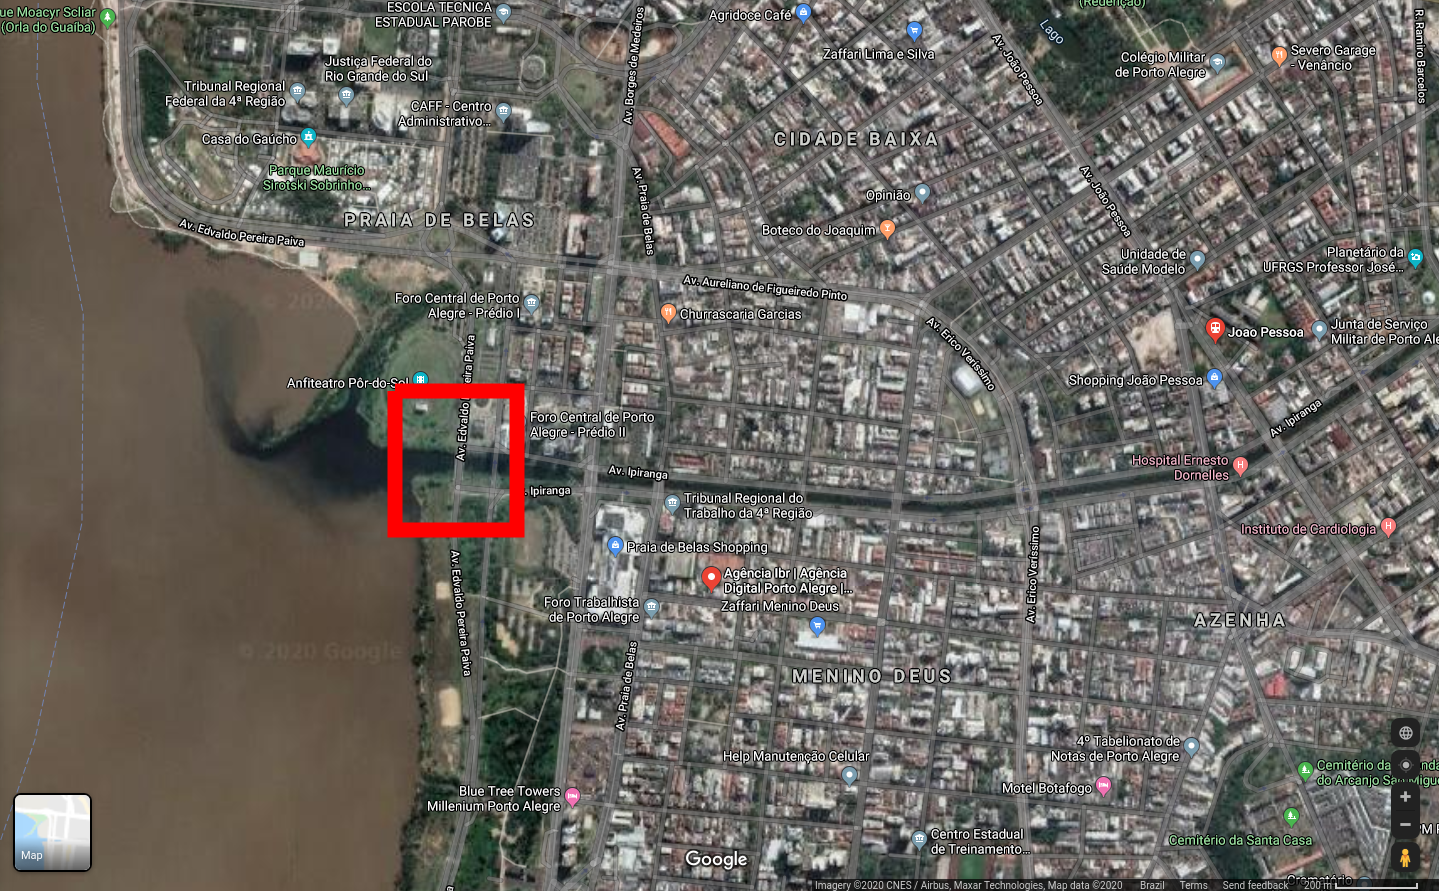
\includegraphics[scale=0.3]{figs/simulation_diluvio_googleLocation_roundedArea.png}
        \caption{Google maps simulation location (-30.047258°, -51.232660°) Av. Edvaldo Pereira Paiva, 1970 - Praia de Belas - Porto Alegre - RS - Brazil}
        \label{fig:simulation_diluvio_googleLocation_roundedArea}
    \end{figure}
    
    \begin{figure}[H]
    \centering
        \begin{subfigure}[b]{0.5\textwidth}
            \centering
            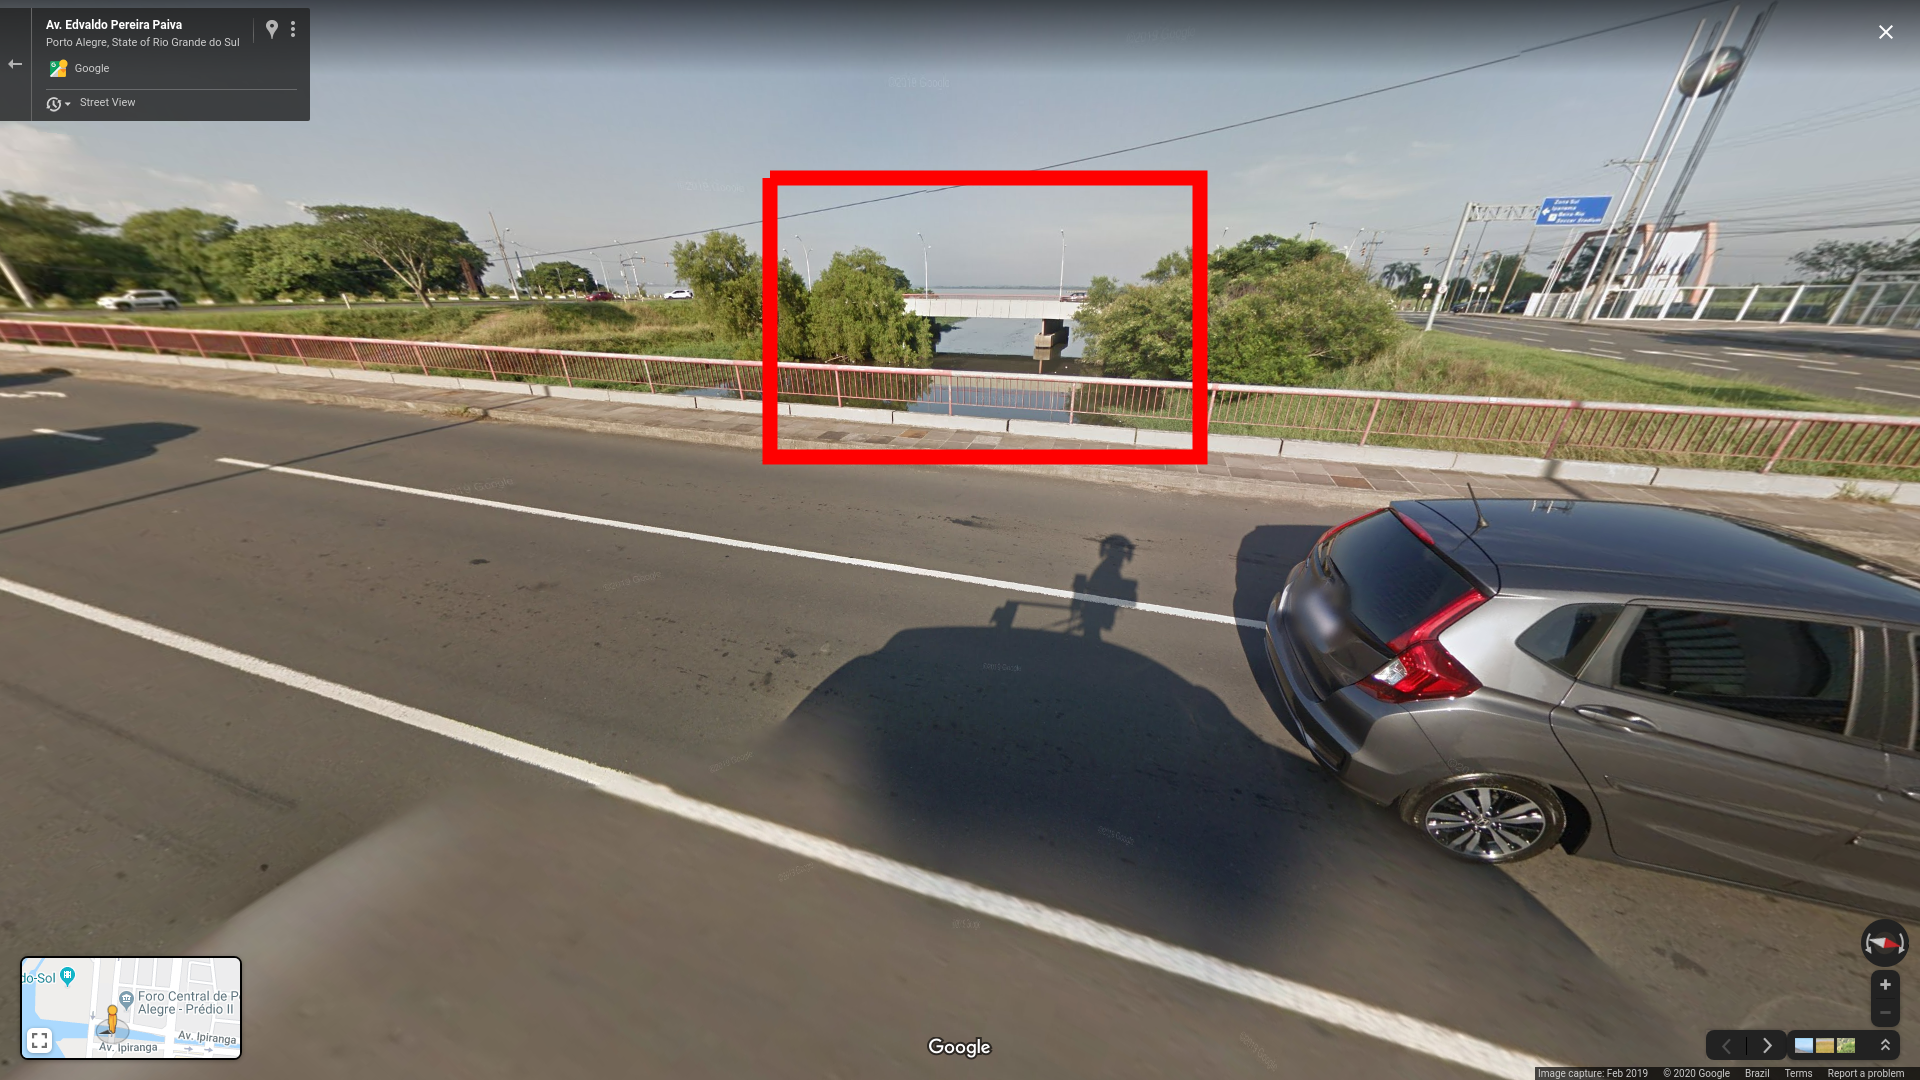
\includegraphics[scale=0.1]{figs/simulation_diluvio_googleLocation2_1_roundedArea.png}
            \caption{Real World}
            \label{fig:simulation_diluvio_googleLocation2_1_roundedArea}
        \end{subfigure}
        \begin{subfigure}[b]{0.4\textwidth}
            \centering
            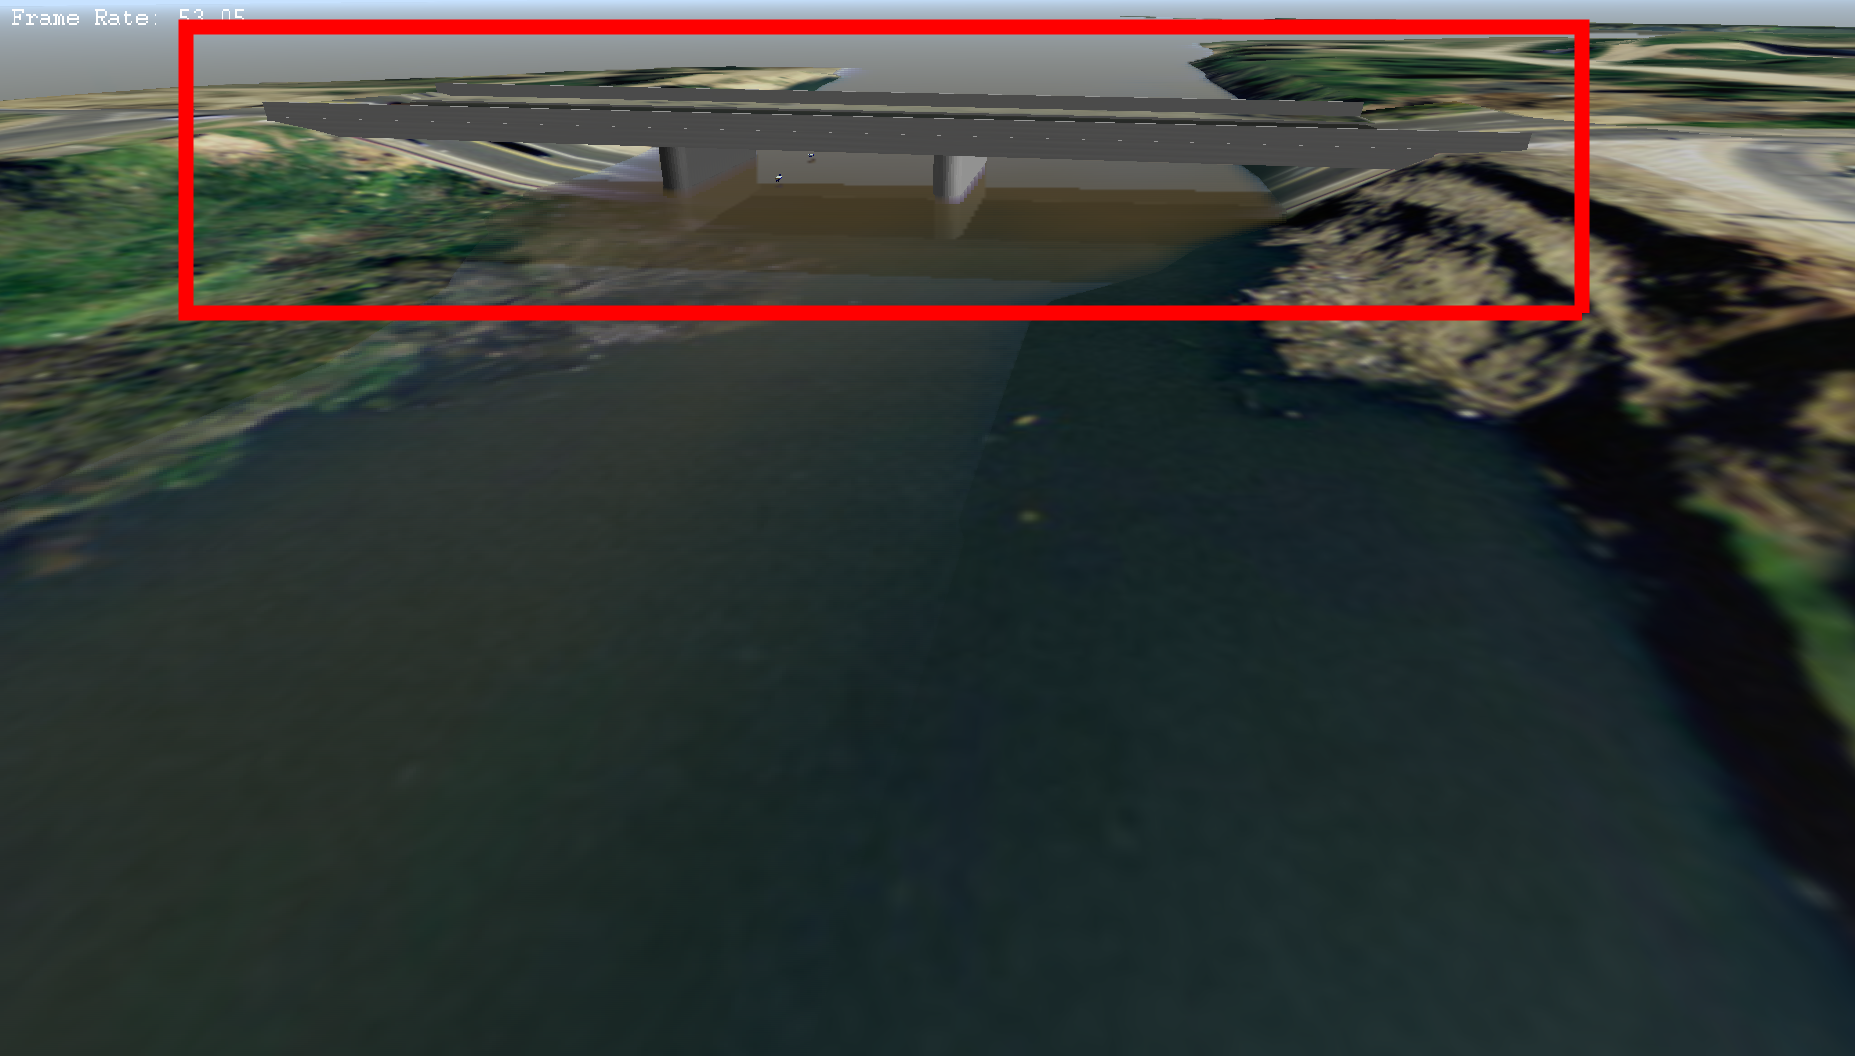
\includegraphics[scale=0.1]{figs/simulation_diluvio_googleLocation2_2_roundedArea.png}
            \caption{Real World Simulated}
            \label{fig:simulation_diluvio_googleLocation2_2_roundedArea}
        \end{subfigure}
    
    \caption{Real world region and its simulated version}
    \label{fig:simulation_diluvio_googleLocation2_roundedArea}
    \end{figure}
    
    % As presented in Chapter \ref{chap:2_TheoreticalBackground}, a head-on scenario is mainly characterized by an encounter between two vessels with a relative bearing of 30°. The assembled scenario is presented in Figure \ref{fig:simulation_uwsim_encounters}.
    
    \begin{figure}[H]
    \centering
    
        \begin{subfigure}[b]{0.5\textwidth}
            \centering
            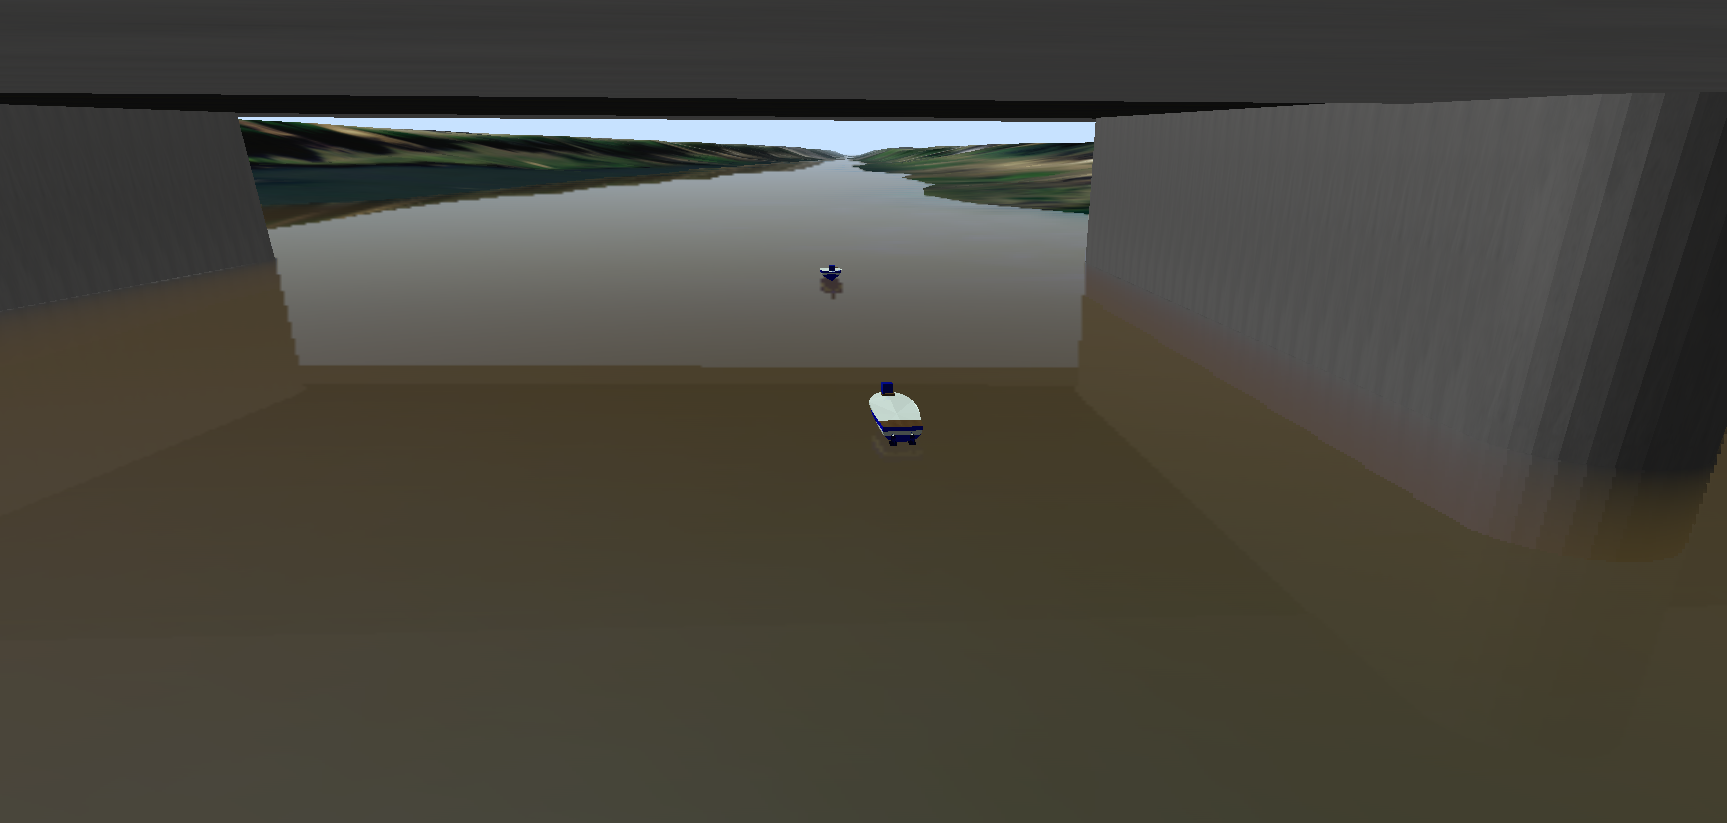
\includegraphics[width=\textwidth]{figs/simulation_uwsim_headon_starting_pos.png}
            \caption{Head On}
            \label{fig:simulation_uwsim_headon_starting_pos}
        \end{subfigure}
        \begin{subfigure}[b]{0.45\textwidth}
            \centering
            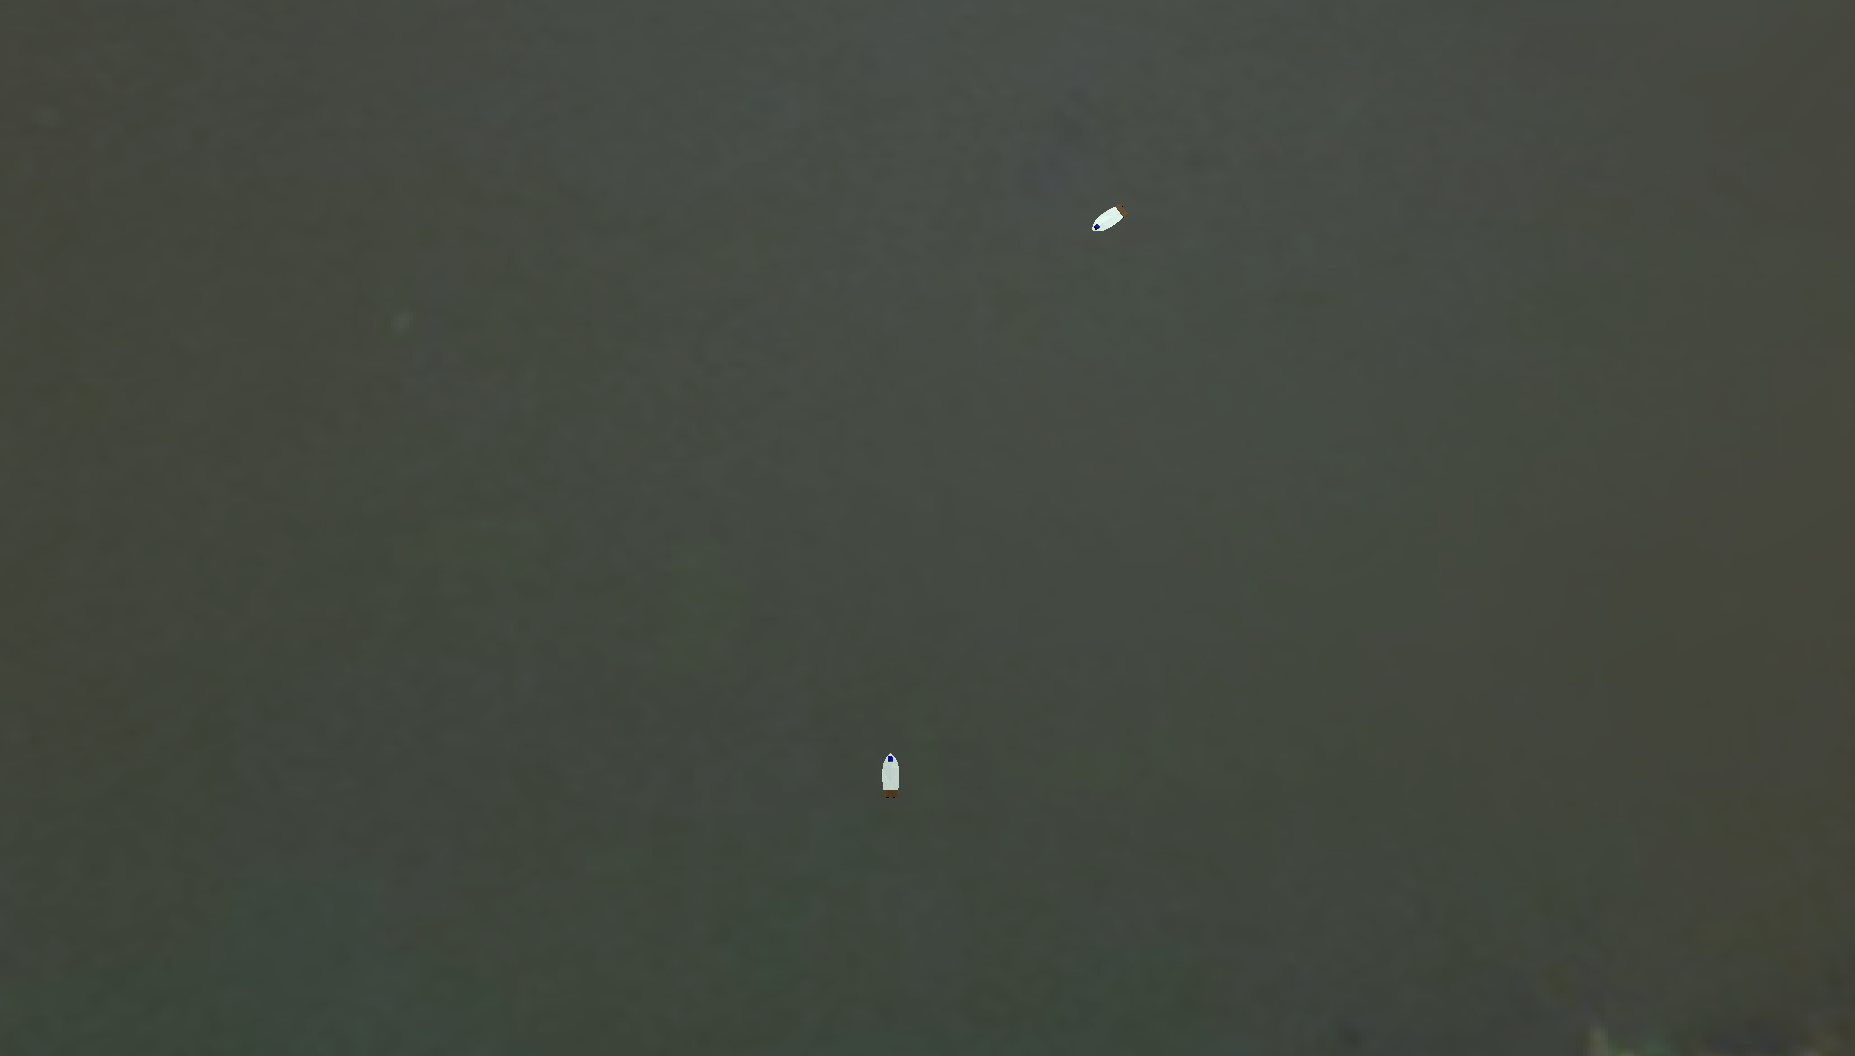
\includegraphics[width=\textwidth]{figs/simulation_uwsim_crossingright_starting_pos.png}
            \caption{Crossing from Right}
            \label{fig:simulation_uwsim_crossingright_starting_pos}
        \end{subfigure}
        
        \begin{subfigure}[b]{0.5\textwidth}
            \centering
            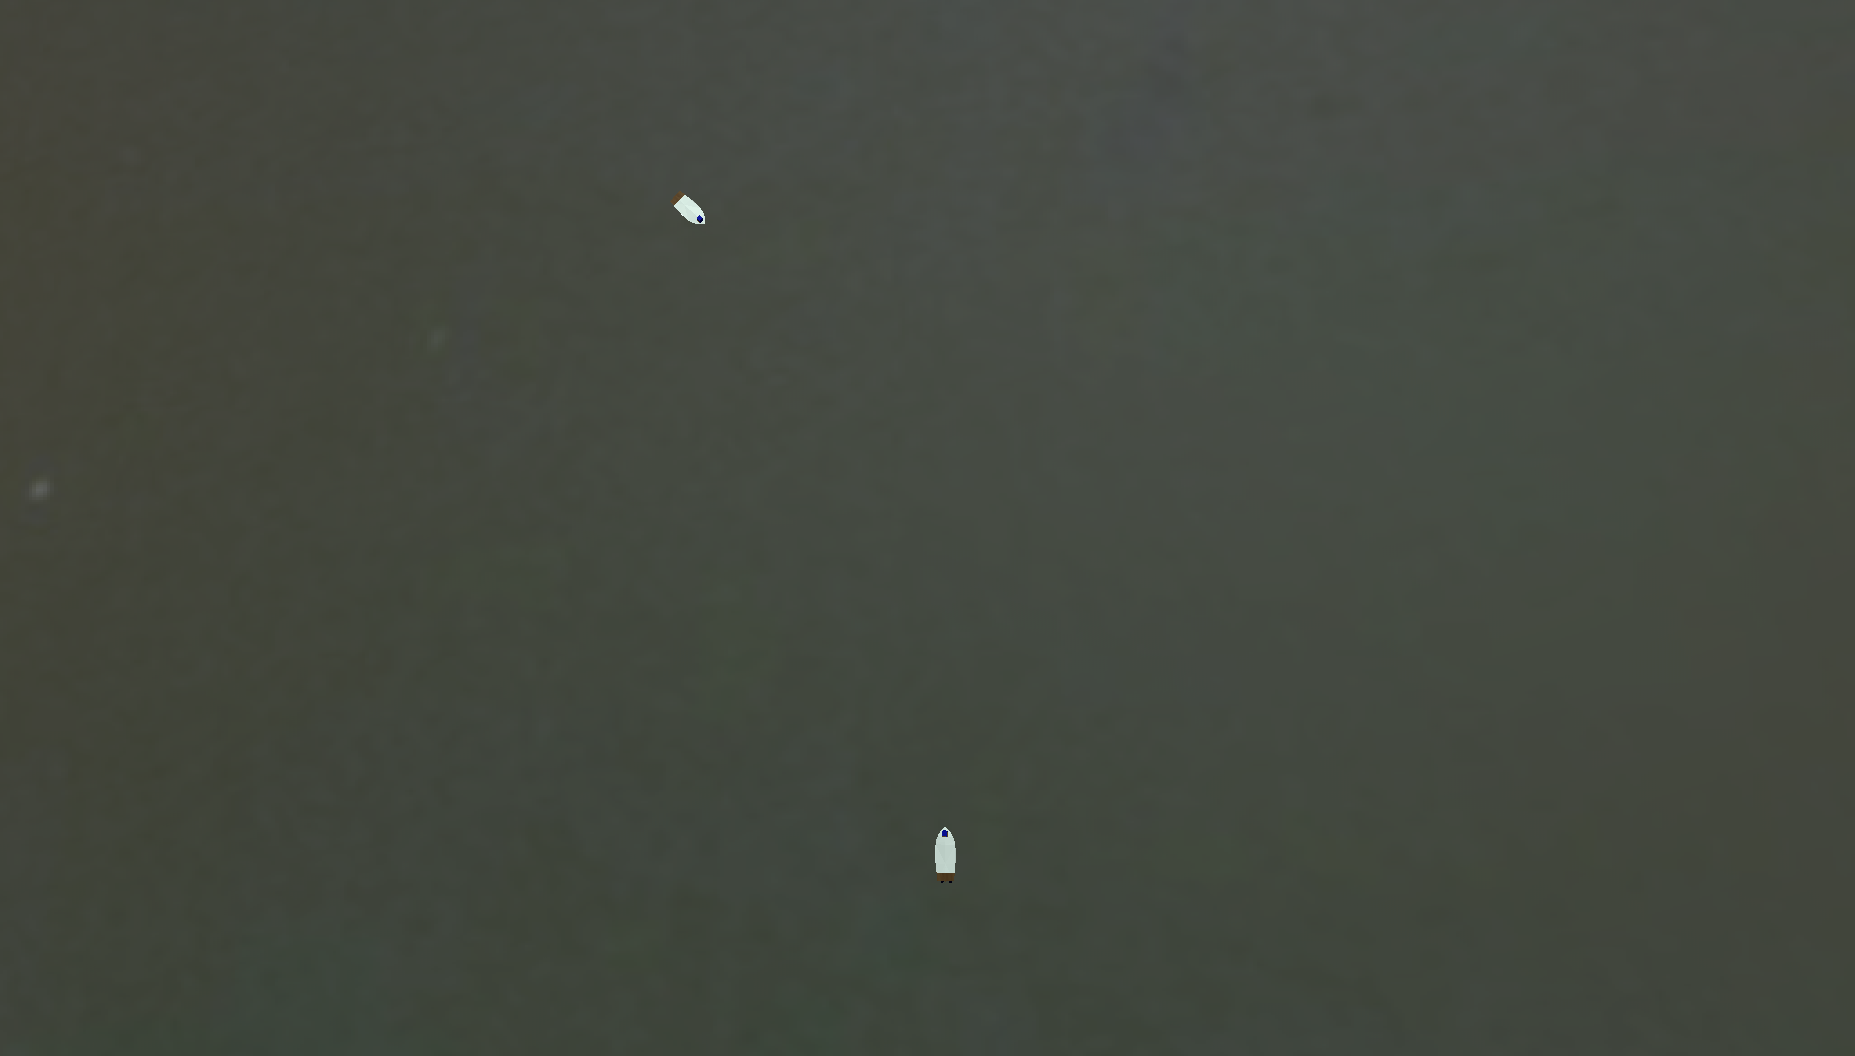
\includegraphics[width=\textwidth]{figs/simulation_uwsim_crossingleft_starting_pos.png}
            \caption{Crossing from Left}
            \label{fig:simulation_uwsim_crossingleft_starting_pos}
        \end{subfigure}
        \begin{subfigure}[b]{0.45\textwidth}
            \centering
            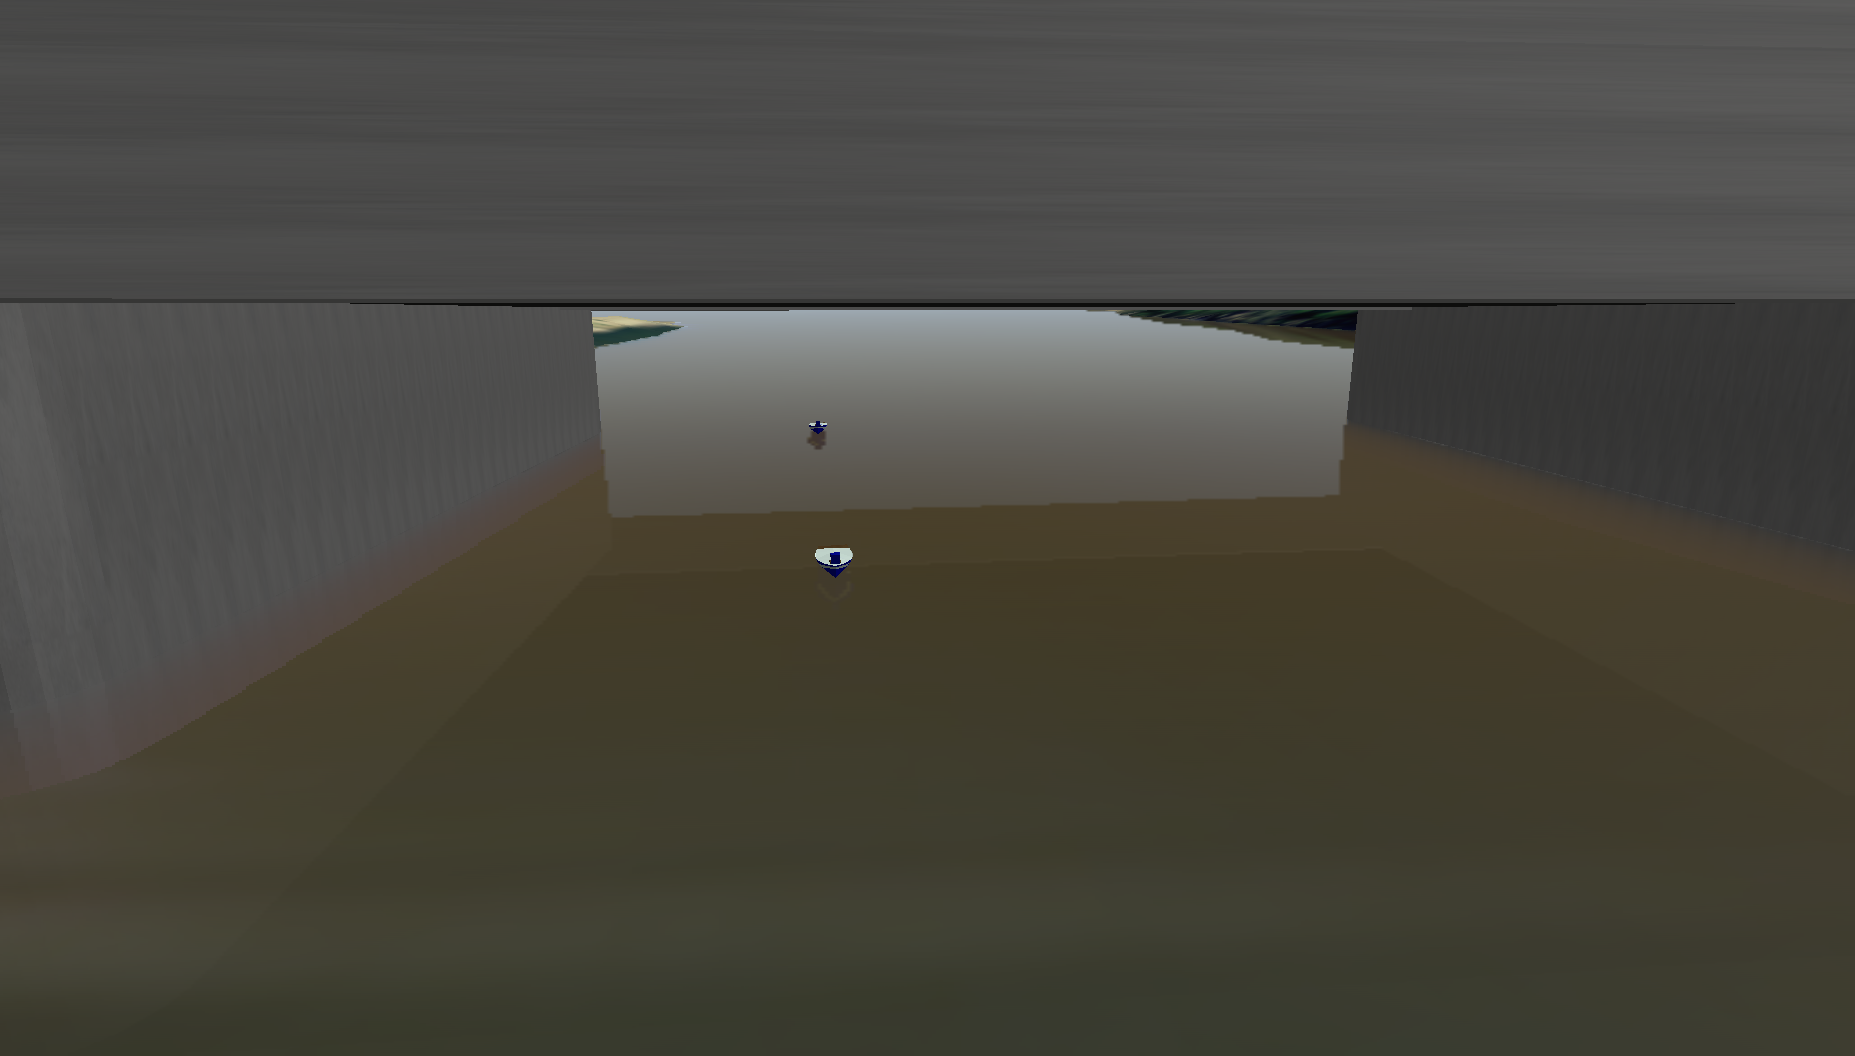
\includegraphics[width=\textwidth]{figs/simulation_uwsim_overtake_starting_pos.png}
            \caption{Overtaking}
            \label{fig:simulation_uwsim_overtake_starting_pos}
        \end{subfigure}
    
    \caption{Encounter scenarios for evaluation. Scenarios adopted from ~\cite{Huang2019Generalized}.}
    \label{fig:simulation_uwsim_encounters}
    \end{figure}
    
    % Please add the following required packages to your document preamble:
    % \usepackage{booktabs}
    \begin{table}[H]
    \centering
    \begin{tabular}{@{}cccc@{}}
        \toprule
        \multicolumn{4}{c}{Own Vessel}                                                                                                                                 \\ \midrule
        \multicolumn{1}{|c|}{}               & \multicolumn{1}{c|}{Initial Pose (m, m, º)} & \multicolumn{1}{c|}{Max. Speed (m/s)} & \multicolumn{1}{c|}{Waypoint}     \\ \midrule
        \multicolumn{1}{|c|}{Head On}        & \multicolumn{1}{c|}{(450, 107.5, 0)}        & \multicolumn{1}{c|}{0.4}              & \multicolumn{1}{c|}{(480, 107.5)} \\ \midrule
        \multicolumn{1}{|c|}{Crossing Right} & \multicolumn{1}{c|}{(410, 105, 90)}         & \multicolumn{1}{c|}{0.86}             & \multicolumn{1}{c|}{(410, 133)}   \\ \midrule
        \multicolumn{1}{|c|}{Crossing Left}  & \multicolumn{1}{c|}{(410, 105, 90)}         & \multicolumn{1}{c|}{0.29}             & \multicolumn{1}{c|}{(410, 133)}   \\ \midrule
        \multicolumn{1}{|c|}{Overtaking}     & \multicolumn{1}{c|}{(450, 107.5, 0)}        & \multicolumn{1}{c|}{0.5}              & \multicolumn{1}{c|}{(550, 107.5)} \\ \midrule
        \multicolumn{1}{l}{}                 & \multicolumn{1}{l}{}                        & \multicolumn{1}{l}{}                  & \multicolumn{1}{l}{}              \\ \midrule
        \multicolumn{4}{c}{Encountering Vessel}                                                                                                                        \\ \midrule
        \multicolumn{1}{|l|}{}               & \multicolumn{1}{l|}{Initial Pose (m, m, º)} & \multicolumn{1}{l|}{Max. Speed (m/s)} & \multicolumn{1}{l|}{Waypoint}     \\ \midrule
        \multicolumn{1}{|c|}{Head On}        & \multicolumn{1}{c|}{(461, 107.5, 180)}      & \multicolumn{1}{c|}{0.15}             & \multicolumn{1}{c|}{(350, 107)}   \\ \midrule
        \multicolumn{1}{|c|}{Crossing Right} & \multicolumn{1}{c|}{(416, 120, 225)}        & \multicolumn{1}{c|}{0.18}             & \multicolumn{1}{c|}{(404, 115)}   \\ \midrule
        \multicolumn{1}{|c|}{Crossing Left}  & \multicolumn{1}{c|}{(416, 120, 315)}        & \multicolumn{1}{c|}{0.44}             & \multicolumn{1}{c|}{(416, 115)}   \\ \midrule
        \multicolumn{1}{|c|}{Overtaking}     & \multicolumn{1}{c|}{(461, 107.5, 0)}        & \multicolumn{1}{c|}{0.15}             & \multicolumn{1}{c|}{(600, 107)}   \\ \bottomrule
        \end{tabular}
    \caption{Encounter scenarios Configuration}
    \label{tab:simulation_scenarios_configuration}
    \end{table}
    
    In our simulations, we use a differential boat - shown in Figure \ref{fig:diffboat} - with two thrusters, which enables it to rotate over its axis. This boat is modeled according to specifications of the Lutra Prop boat, acquired from Platypus ~\cite{PlatypusLLC}. The differential boat is 106 centimeters long, 48 centimeters wide and 15 centimeters tall, being able to achieve a maximum speed of 1.14 m/s. In its bow, we simulate a parameterized laser for environment scanning, allowing us to set different angles and detection distance ranges.
    
    \begin{figure}[H]
        \centering
        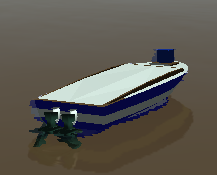
\includegraphics[scale=0.75]{figs/diffboat.png}
        \caption{Simulated version of Lutra Prop boat}
        \label{fig:diffboat}
    \end{figure}
    
    Agrawal \etal ~\cite{Agrawal2015COLREGS} evaluate theirs A* approach in a 100mx100m grid with a resolution of 1:1, resulting in a search space of 10000 cells, our scenarios were built respecting the same proportionality. In all scenarios, our \ac{USV} plan in a 20mx20m grid with 1:0.2 resolution, resulting in a search space of 10000 cells. The choice of 20x20 dimension is related to real limitations of the range and reliability on laser sensors, the RPLIDAR A3 laser~\cite{RPLidarA3} model, for example, is reliably capable of detection in a 25 meters distance range.
    
    \section{Experiments Results}
    
        As presented before we adopted scientific experimentation for \ac{ATC} correctness evaluation, running same scenario twice, one execution with \ac{ATC} and another without \ac{ATC}. Results and their respective description for head on and crossing from right scenarios are presented respectivelly in Figures \ref{fig:Result_HeadOn_With_Without_ATC} and \ref{fig:Result_CrossingRight_With_Without_ATC}. For each scenario, we measured the computation time of every execution of our path planner, average sustained speed, and minimal distance maintained between the vessels, and evaluated successful avoidance. In Table \ref{tab:results} we show collected results.
        
        \begin{figure}[H]
            \centering
            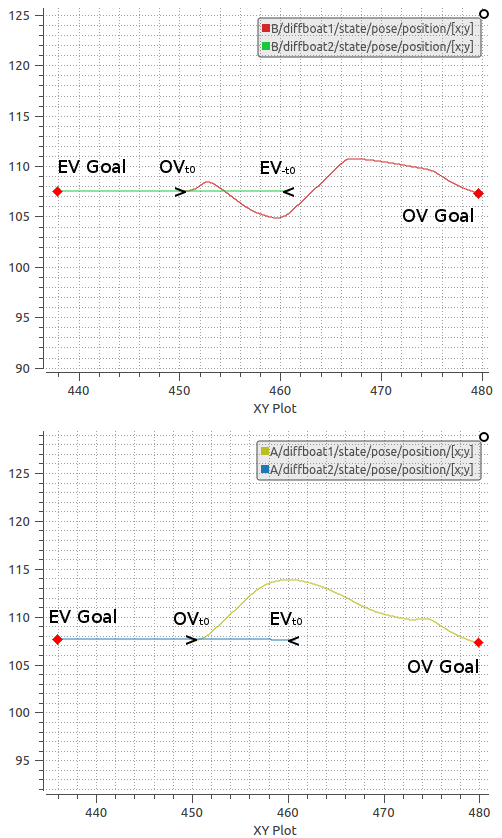
\includegraphics[scale=0.50]{figs/Result_HeadOn_With_Without_ATC.png}
            \caption{Head-on Scenario Simulation Result with \ac{ATC} vs without \ac{ATC}. Start positions are denoted by OV$_{t0}$ for own vessel and EV$_{t0}$ for encountering vessel. (A) Own vessel COLREGS-compliant behavior due to A* \ac{ATC} path planner. (B) Non COLREGS-compliant own vessel behavior generated by A* without \ac{ATC}.}
            \label{fig:Result_HeadOn_With_Without_ATC}
        \end{figure}
        
        \begin{figure}[H]
            \centering
            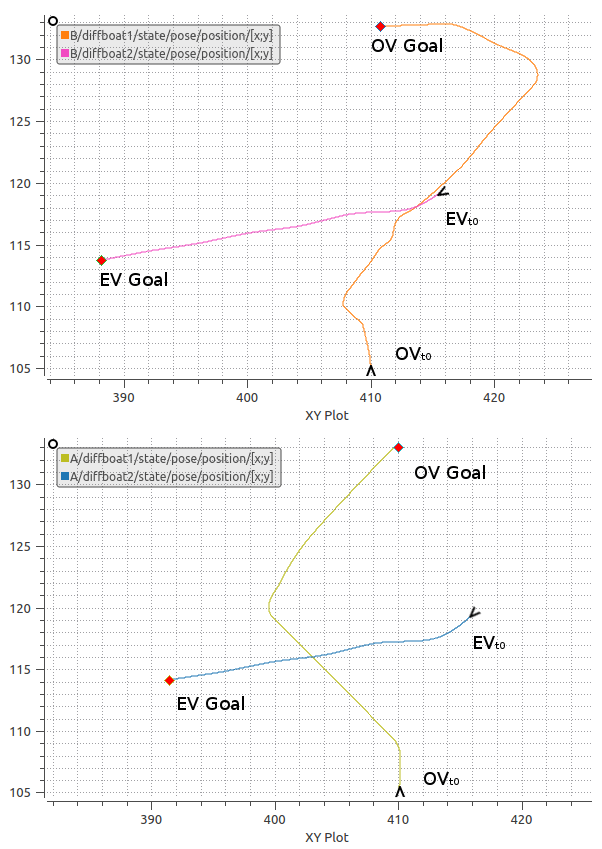
\includegraphics[scale=0.50]{figs/Result_CrossingRight_With_Without_ATC.png}
            \caption{Crossing from Right Scenario Simulation Result with \ac{ATC} vs without \ac{ATC}. Start positions are denoted by OV$_{t0}$ for own vessel and EV$_{t0}$ for encountering vessel. (A) Own vessel COLREGS-compliant behavior due to A* \ac{ATC} path planner. (B) Non COLREGS-compliant own vessel behavior generated by A* without \ac{ATC}.}
            \label{fig:Result_CrossingRight_With_Without_ATC}
        \end{figure}
        
% \usepackage{multirow}


\begin{table}
\centering
\begin{tabular}{|c|c|c|c|c|c|c|} 
\hline
\multirow{2}{*}{\textbf{Encounter} }                                                               & \multirow{2}{*}{\begin{tabular}[c]{@{}c@{}}\textbf{Scenario }\\\textbf{ Variation} \end{tabular}} & \multicolumn{3}{c|}{\begin{tabular}[c]{@{}c@{}}\textbf{Computational }\\\textbf{ Time (s)} \end{tabular}} & \multirow{2}{*}{\begin{tabular}[c]{@{}c@{}}\textbf{Successful }\\\textbf{ Avoidance} \end{tabular}} & \multirow{2}{*}{\begin{tabular}[c]{@{}c@{}}\textbf{Minimum }\\\textbf{ Distance (m)} \end{tabular}}  \\ 
\cline{3-5}
                                                                                                   &                                                                                                   & \textbf{Max.}  & \textbf{Average}  & \textbf{Std. Deviation}                                              &                                                                                                     &                                                                                                      \\ 
\hline
\multirow{3}{*}{\textbf{Head-On} }                                                                 & \textbf{No ATC}                                                                                   & 0.369          & 0.074             & 0.081                                                                & Yes                                                                                                 & 4.431                                                                                                \\ 
\cline{2-7}
                                                                                                   & \textbf{ATC}                                                                                      & 0.364          & 0.076             & 0.076                                                                & Yes                                                                                                 & 1.599                                                                                                \\ 
\cline{2-7}
                                                                                                   & \textbf{Wind}                                                                                     & 0.355          & 0.077             & 0.079                                                                & Yes                                                                                                 & 1.505                                                                                                \\ 
\hline
\multirow{3}{*}{\begin{tabular}[c]{@{}c@{}}\textbf{Crossing }\\\textbf{ from Right} \end{tabular}} & \textbf{No ATC}                                                                                   & 0.390          & 0.050             & 0.098                                                                & Yes                                                                                                 & 5.4145                                                                                               \\ 
\cline{2-7}
                                                                                                   & \textbf{ATC}                                                                                      & 0.395          & 0.052             & 0.104                                                                & Yes                                                                                                 & 3.264                                                                                                \\ 
\cline{2-7}
                                                                                                   & \textbf{Wind}                                                                                     & 0.403          & 0.085             & 0.124                                                                & Yes                                                                                                 & 3.739                                                                                                \\ 
\hline
\multirow{3}{*}{\begin{tabular}[c]{@{}c@{}}\textbf{Crossing }\\\textbf{ from Left} \end{tabular}}  & \textbf{No ATC}                                                                                   & 0.003          & 0.001             & 0.0003                                                               & Yes                                                                                                 & 2.881                                                                                                \\ 
\cline{2-7}
                                                                                                   & \textbf{ATC}                                                                                      &                &                   &                                                                      &                                                                                                     &                                                                                                      \\ 
\cline{2-7}
                                                                                                   & \textbf{Wind}                                                                                     &                &                   &                                                                      &                                                                                                     &                                                                                                      \\ 
\hline
\multirow{3}{*}{\textbf{Overtaking} }                                                              & \textbf{No ATC}                                                                                   &                &                   &                                                                      &                                                                                                     &                                                                                                      \\ 
\cline{2-7}
                                                                                                   & \textbf{ATC}                                                                                      & 0.357          & 0.018             & 0.022                                                                & Yes                                                                                                 & 3.101                                                                                                \\ 
\cline{2-7}
                                                                                                   & \textbf{Wind}                                                                                     & 0.852          & 0.039             & 0.073                                                                & Yes                                                                                                 & 1.787                                                                                                \\
\hline
\end{tabular}
\label{tab:results}
\end{table}